\documentclass[
 reprint,
%superscriptaddress,
%groupedaddress,
%unsortedaddress,
%runinaddress,
%frontmatterverbose, 
%preprint,
%preprintnumbers,
%nofootinbib,
%nobibnotes,
%bibnotes,
 amsmath,amssymb,
 aps,
%pra,
%prb,
%rmp,
%prstab,
%prstper,
%floatfix,
]{revtex4-2}

\usepackage{colortbl}
\usepackage{graphicx} 
\usepackage{booktabs}
\usepackage{caption}
\usepackage{notes2bib}
\newcommand{\red}{\textcolor{red}}

\begin{document}

\title{Beyond May: Complexity-stability relationships \\
in high-dimensional dynamical systems}

\author{Onofrio Mazzarisi}
\author{Matteo Smerlak}

 \affiliation{MPI MiS}


\date{\today}% It is always \today, today,
             %  but any date may be explicitly specified

\begin{abstract}
Fifty years ago, Robert May predicted that large, complex systems are unlikely to be stable. Here, we revisit May's argument to show that there are, in fact, two kinds of complexity-stability relationships in disordered dynamical systems, depending on the relative convexity of the response to self- vs. cross-interactions. We illustrate the transition between "May" (complexity begets instability) and "anti-May" (complexity begets stability) behavior with a non-linear generalization of the Lotka-Volterra model. 
\end{abstract}

\maketitle

\section{Introduction}

Few mathematical arguments have influenced biological thinking like May's
prediction that large, complex systems cannot be stable~\cite{May1972}. 
It is, on the face of it, a perplexing conclusion. 
On the one hand, May's argument is so simple and compelling
that it hard not to conclude that it must hold universally,
and beyond biology~\cite{Haldane2011,Moran2019}. 
On the other, it is clear that at least some large, 
complex systems are stable---or else which stable patterns 
would ecology be studying in the first place? If anything, 
the opposite relationship between complexity and stability 
seems to hold empirically: rich, strongly coupled ecosystems 
(eg. rainforests) tend to be  stable over time, while sparser ones 
(eg. arctic environments) often exhibit large fluctuations, 
exctinctions, and invasions~\cite{Loreau2022,McCann2000,Hutchinson1959,Odum1959,MacArthur1955}. 

May's argument goes as follows. A system with $N$ populations $x_i$ is stable 
is one that can be characterized by an equilibrium point $x^*$. 
Near that equilibrium $x = x^* + \delta x$, the 
dynamics of the system will be described by linear 
equations $d(\delta x)/dt = A (\delta x)$, and stability of 
these equations requires that all eigenvalues of $A$ 
have negative real part. But if $A$ can be represented as $A = B - I$, 
where $B$ consists of random, independent interactions with zero 
mean and variance $\sigma^2$, and $-I$ corresponds to 
stabilizing self-interactions on some natural timescale, 
then the circular law of random matrix theory implies that all 
eigenvalues of $A$ will have negative real part only if $\sigma^2 N < 1$. 
This places a sharp constraint on both diversity $N$ and interaction 
strengh $\sigma$, often referred to as "complexity begets instability". 
(This argument generalizes to $\langle B_{ij}\rangle \neq 0$, 
to incomplete connectivity, or to correlated interactions.)

In ecology, many authors have sought to ease the tension between May's 
prediction and empirical observation by invoking effects not captured by 
dynamical systems with random 
coefficients~\cite{McCann2000,Chesson2000,Mougi2012,Rohr2014,Barabas2017,Grilli2017}. 
Here, we show that May's argument is itself incomplete: 
random dynamical systems do not necessarily imply that 
stability decreases with diversity or interaction 
strength---the opposite behavior is also possible, 
without the need for special or additional structure. 

\section{Results}

\subsection{Model}

Consider the dynamical system in $N$ variables
\begin{equation}\label{dynamics}
    \dot{x}_i = f(x_i) + \sum_{j}a_{ij}g(x_i)h(x_j) \, .
\end{equation}
Here $f(x_i)$ represents the self-dynamics of a population $i$, while $g(x_i)$ and $h(x_j)$ capture the interaction of $i$ with other populations. 
That interaction is weighted by a coefficient $a_{ij}$, such that $a_{ij} > 0$ (resp. $a_{ji} < 0$) implies a positive (resp. negative) effect of $j$ on the growth of $i$. 
In the following we refer to $f(x_i)$ as the ``production function'' and $g(x_i)$ as the ``response function''. 
This rather general setting has been used to study universality\cite{Barzel2013} and to construct 
minimal models for complex dynamics\cite{Barzel2015} ranging from biological~\cite{Alon2006,Karlebach2008,Skinner2012} 
to social~\cite{Pastor-Satorras2001,Hufnagel2004,Dodds2005} systems. 

The classic generalized Lotka-Volterra (GLV) competition model corresponds to $f$, $g$, $h$ all linear. 
However, it is natural both physically and biologically to consider more general functions, including power laws $f(x)\sim x^\alpha$, $g(x)\sim x^\beta$, $h(x) \sim x^\gamma$. 
From a physical perspective, we can imagine populations $x_i$ forming three-dimensional clusters whose growth is limited to their two-dimensional surface, leading to a production function $f(x) \sim x^{2/3}$. 
Biologically, the growth of organisms (populations of cells) has long been known to scale like $f(x) \sim x^k$ with $k\simeq 3/4$~\cite{Brown2004}, which can be understood in terms of hydrodynamic constraints on vascular and pulmonary networks. 
For reasons that are not currently understood, a similar pattern of growth appears to recur at the community level~\cite{Hatton2015,Hatton2023}. 
It has recently been shown appropriate to model predator-prey interactions with a square root laws ($g(x) \sim h(x) \sim x^{1/2}$)~\cite{Barbier2021,Mazzarisi2023}, for example. 

\subsection{Homogeneous interactions}

Under what condition does \eqref{dynamics} admit a linearly stable equilibrium? We begin by considering the simple case where all self-interactions have the same strength $a_{ii} = a_{\textrm{s}}$, and similarly for cross-interactions $a_{ij} = a_{\textrm{c}}$ ($i\neq j$). Under these assumptions, a straightforward computation shows that an equilibrium $x_*$ will be linearly stable if  
\begin{equation}\label{homogeneous-general}
    \left(\frac{f'_*}{f_*} - \frac{g'_*}{g_*}\right) + (a_{\textrm{s}} - a_{\textrm{c}})\,\frac{g_*h'_*}{f_*} < 0. 
\end{equation}
Thus, the stability of a competitive equilibrium depends on the relative strength of self- and cross-interactions ($a_{\textrm{s}} - a_{\textrm{c}}$), but also on the relative convexity of the production and response functions ($f'_*/f_* - g'_*/g_*$). With power laws, \eqref{homogeneous-general} evaluates to 
\begin{equation}
    (\alpha - \beta)(N-1) < \gamma(a_{\textrm{s}}/a_{\textrm{c}}- 1) - (\alpha - \beta)(a_{\textrm{s}}/a_{\textrm{c}}),
\end{equation}
leading to three different regimes:
\begin{itemize}
    \item If $\alpha = \beta$, stability requires $a_{\textrm{s}} > a_{\textrm{c}}$, i.e. self-interactions must be stronger than cross-interactions. This is the usual conclusion drawn from the Lotka-Volterra model. 
    \item If $\alpha > \beta$, stability places an upper bound on $N$: the more complex the system, the less likely to be stable. 
    We can call this "May" behavior.
    \item If $\alpha < \beta$, stability places an lower bound on $N$: the more complex the system, the more likely to be stable. This is "anti-May" behavior.
\end{itemize}

\subsection{Random interactions: general reults}

Consider now Eq.~\eqref{dynamics} with i.i.d. random 
interactions $a_{ij}$ with mean $\mu$ and standard 
deviation $\sigma$, with the diagonal elements $a_{ii}$ 
extracted from a distribution with mean $\mu_s$ 
possibly different from $\mu$ and same standard deviation
as for the off-diagonal elements.  
We can compute the Jacobian matrix at equilibrium
\begin{align}
    J_{ij}^* & = a_{ij}g_*(x_i)h_*'(x_j) \qquad \qquad \textrm{for} \ i\neq j \label{eq: jac off-diag}\\
    J_{ii}^* & = f_*'(x_i) - \frac{g_*'(x_i)f_*(x_i)}{g_*(x_i)} - a_{ii}g_*(x_i)h_*'(x_j) \ , \label{eq: jac diag}
\end{align}
where we used $\sum_{j}a_{ij}g_*(x_i)h_*(x_j)=-f_*(x_i)/g_*(x_i)$.
In order to investigates its spectral properties, 
we follow Stone~\cite{Stone2018} and use a
result in random matrix theory~\cite{Ahmadian2015}
which generalize the classical `circular law'~\cite{Potters2020}.

In Ref.~\cite{Ahmadian2015} Ahmadian \emph{et al.} 
consider matrices of the form $M + LSR$, where $M$,  
$L$ and $R$ are deterministic matrices, and $S$ 
is a random matrix with i.i.d. coefficients, 
zero mean and variance $\sigma^2$. They 
show that in the complex plane the boundary of the 
eigenspectrum of large matrices of this form is defined by
$\textrm{Tr}[(M_\zeta M_\zeta^\dagger)^{-1}]\geq \sigma^{-2}$ , 
where $M_\zeta = L^{-1}(\zeta I - M)R^{-1}$ and $\zeta\in\mathbb{C}$. 
If $L$, $R$ and $M$ are all diagonal $N\times N$ matrices, 
this condition simplifies to
\begin{equation}
    \sum_{i=1}^N\frac{(L_{i}R_{i})^2}{ \vert \zeta - M_{i}\vert^2 }\geq \sigma^{-2} \ .
\label{eq: domain}
\end{equation}

Now we decompose the interaction matrix as
$a = \mu \mathbf{1} + (\mu_s-\mu)I + S$,
with $\mathbf{1}$ the rank-one matrix with all entries equal to $1$
and $S$ a random matrix as defined above.
We can limit ourselves to consider 
$a = (\mu_s-\mu)I + S$ by relying on 
rank-one perturbation theory: we would only neglect outliers
uninfluential for the linear stbaility properties of the system (see Ref.~\cite{Stone2018}).
The Jacobian in Eqs.~\eqref{eq: jac off-diag} and \eqref{eq: jac diag} assumes therefore the form $M + LJR$ with
\begin{align}
    M & = \textrm{diag}\left(f_*'(\mathbf x) -
    \frac{g_*'(\mathbf x)f_*(\mathbf x)}{g_*(\mathbf x)}
    +(\mu_s-\mu)g_*(\mathbf x)h_*'(\mathbf x)\right) \ , \\
    L &= \textrm{diag}(g_*(\mathbf x)) \ , \qquad  
    R = \textrm{diag}(h_*'(\mathbf x)) \ . \nonumber
\end{align}
The domain of the eigenvalues of $J^*$, defined by
Eq.~\eqref{eq: domain}, 
first touches the right half-plane at $\zeta = 0$, 
hence linear stability requires   
\begin{equation}\label{eq: random-stability}
    \sum_{i=1}^N \cfrac{\left(\cfrac{g_*(x_i)h_*'(x_i)}{f_*(x_i)}\right)^2}{
        \Bigl |\left(\cfrac{f_*'(x_i)}{f_*(x_i)} -
        \cfrac{g_*'(x_i)}{g_*(x_i)}\right)
        +(\mu_s-\mu) \cfrac{g_*(x_i)h_*'(x_i)}{f_*(x_i)} \Bigl |^2}
    < \sigma^{-2}. 
\end{equation}
This expression can be considered the
generalization to random interaction of
the expression in Eq.~\eqref{homogeneous-general},
which appears again in the denominator of the summand.

There are straightforward results that follows.
For generalized Lotka-Volterra (GLV) models,
i.e. $f(x_i)=x_i$, $g(x_i)=x_i$ and $h(x_i)=x_i$,
the expression in Eq.~\eqref{eq: random-stability}
becomes independent on the equilibria and we 
recover the linear stability condition
$\sigma\sqrt{N} < (\mu_s-\mu)$.
Moreover we can define an equivalence class of models
which share the same simple condition
for linear stability defined by the equivalence relation
\begin{equation}\label{eq: equiv class glv}
    \left(\cfrac{f_*'(x_i)}{f_*(x_i)} -
        \cfrac{g_*'(x_i)}{g_*(x_i)}\right)\Bigl/
        \cfrac{g_*(x_i)h_*'(x_i)}{f_*(x_i)}=c \ ,
\end{equation}
where $c$ is a constant,
resulting in the condition $\sigma\sqrt{N} < (\mu_s-\mu) +c$.

In the general case in which the dependence on the equilibria
$\mathbf{x}_*$ does not cancel out, it is not possible to
obtain an explicit and simple complexity-stability relationship.
We can make progress in the large $N$ limit by
trasforming the sum in an integral 
$\sum_{i=1}^N\to N\int dx_*P(x_*)$, where $P(x_*)$ 
is the equilibrium distribution of the system
depending on the statistic of the interactions,
and write
\begin{equation}\label{eq: random-stability int}
    \int dx_* \cfrac{NP(x_*) \left(\cfrac{g_*(x)h_*'(x)}{f_*(x)}\right)^2}{
        \Bigl |\left(\cfrac{f_*'(x)}{f_*(x)} -
        \cfrac{g_*'(x)}{g_*(x)}\right)
        +(\mu_s-\mu) \cfrac{g_*(x)h_*'(x)}{f_*(x)} \Bigl |^2}
    < \sigma^{-2} \ .
\end{equation}
This expression allows us to obtain insights on the stability properties of
the system in the case in which we are able to compute or estimate 
the probability distribution function $P(x_*)$.

\subsection{Random interactions: power laws case}
In order to investigate the different regimes
of complexity-stability behaviour,
let us specialize to the power laws case, with 
\begin{equation}
    f(x_i)=x_i^{\alpha} \ , \quad g(x_i)=-x_i^{\beta} \ , \quad h(x_i)=x_i^{\gamma} \ .
\end{equation} 
Additional proportionality constants can be reabsorbed in the statistics
of $a$ and by a rescaling of time, moreover we chose to explicitly
factor out a minus sign in order to more straightforwardly connect
with competitive models.

We wish to consider explictly cases
for "May" and "anti-May" regimes.
An example of the former is given by GLV.
In order to explore the latter, we 
need to resort to Eq.~\eqref{eq: random-stability int} and therefore
to compute the equilibrium probability distribution function
for the system. This can be achieved in different ways,
depending, among other things, on specific constraints 
imposed on the system. 
One approach is reported below, 
then we specialize to a specific choice of 
the power laws exponents.

Following, e.g., Ref.~\cite{Roy2019} we can derive from 
the evolution equation
\begin{equation}
    \dot{x_i}=x_i^{\alpha} - x_i^{\beta}\sum_{j}a_{ij}x_j^{\gamma} \, ,
\label{eq: full abg}
\end{equation}
for large $N$, a dynamical mean field theory (DMFT) 
describing the entire ensemble of $N$ variables
thorugh the evolution of the representative random variable $x$
\begin{equation}
    \dot{x} = x^{\alpha}-a_sx^{\beta+\gamma}-x^{\beta}\left( \mu N \langle x^{\gamma}\rangle + \sigma \sqrt{N} \eta\right) \, ,
\label{eq: dmft}
\end{equation}
where $a_s$ is a random variable with the statistics of $a_{ii}$,
$\langle . \rangle$ stands for expectation value
and $\eta$ is a gaussian variable
with zero mean and correlation 
$\langle x^{\gamma}(t)x^{\gamma}(s)\rangle$. 
The averages and correlations have to be computed self-consistently.
If the system admits an equilibrium, for 
$t\to\infty$ each of the initial $N$ degrees 
of freedom will reach a final finite value. 
The effective random variable describing their statistics
also become time-independent,
$\lim_{t\to\infty}x(t)=x_*$ and we can write
\begin{equation}
    x_*^{\alpha-\beta} - a_s x_*^{\gamma}= \left( \mu N \langle x_*^{\gamma}\rangle + \sigma \sqrt{N\langle x_*^{2\gamma}\rangle}\xi\right) \, ,
\end{equation} 
where $\xi$ is a standard normal random variable (i.e. $\xi\sim\mathcal{N}(0,1)$).
The equation above can be solved for $x_*$ for specific values of
$(\alpha-\beta)/\gamma$, or, in general, if we set $a_s=0$, which amounts to include
all the self-interaction in the nonlinear produciton term
$x_*^{\alpha}$. In the following, for cases which
falls in the "anti-May" phase, we show that numerical results
for non-vanishing diagonal part of the
interaction matrix and equal to the
off-diagonal part are well approximated by the results obtained
setting $a_s=0$.

In this case the stationary solution is given by 
\begin{equation} \label{eq: cavity solution}
    x_* = \left( \mu N \langle x_*^{\gamma}\rangle + \sigma \sqrt{N\langle x_*^{2\gamma}\rangle}\xi\right)^{1/(\alpha-\beta)} \, .
\end{equation}
The equilibrium probability distribution function for $x_*$, $P(x_*)$,
can be obtained as the pushforward of the distribition of $\xi$.
The change of measure
$\left|d \xi/d x_*\right|=|\alpha-\beta|x_*^{\alpha-\beta-1}/\sigma \sqrt{N\langle x_*^{2\gamma}\rangle}$,
leads to
\begin{equation}\label{eq: dist general}
    P(x_*)=\frac{|\alpha-\beta|x_*^{\alpha-\beta-1}}{\sqrt{2\pi\sigma^2 N\langle x_*^{2\gamma}\rangle}}
    \exp{\left\{-\frac{(x_*^{\alpha-\beta}-\mu N\langle x_*^{\gamma}\rangle)^2}{2\sigma^2N\langle x_*^{2\gamma}\rangle}\right\}} \, ,
\end{equation}
where the expectations have to be computed self-consistently.

Let us focus on the specific choice 
$\alpha=1$, $\beta=1.5$ and $\gamma=1$, with
$a_s=0$ in order to leverage the equilibrium solution in Eq.~\eqref{eq: dist general}.
In this case the first and second moments, 
to be self-consistently computed, formally diverges. This is not truly porblematic in practice
because we are dealing with large, but \emph{finite} populations.
Following~\cite{Cui2020,Hatton2023} and assuming
$\sigma \sqrt{N\langle x_*^2\rangle}\ll \mu N \langle x_* \rangle$,
we can Taylor expand to the first-order in 
$\sigma \sqrt{N\langle x_*^2\rangle}$ the cavity 
solution~\eqref{eq: cavity solution} and 
approximate to Eq.~\eqref{eq: dist general} with
a gaussian distribuiton
with moments $\langle x_*\rangle=(\mu N)^{-2/3}$ and
$\langle x_*^2\rangle=(\mu N)^{-4/3}/(1-4(\mu N)^{-2}\sigma^2N)$.

The result is plotted against simulations in 
Fig.~\ref{fig: cavity sol.}, alongside the exact 
solution~\eqref{eq: dist general} 
where integration for the moments has been performed up to a maximum
value above which no equilibirum value should 
be found, for a given $N$.
Simulations correspond to $a_s=\mu$, showing that the choice
of vanishing self-interaction for the analytical results
is suited to describe this case as well.

\begin{figure}[h!]
    \centering
    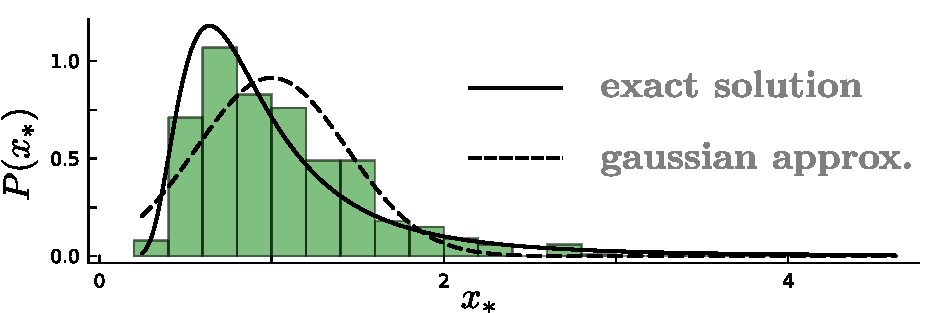
\includegraphics[width=.45\textwidth]{figs/cavity.pdf}
    \caption{The equilibrium distribution for a realization
    of the system described by Eq.~\eqref{eq: full abg} 
    is accurately reproduced by the cavity solution in 
    Eq.\eqref{eq: dist general} and its gaussian approximation.
    For the simulation we used  $\alpha=1$, $\beta=1.5$,
    $\gamma=1$, $N=50$, $\mu=\mu_s=10^{-2}$, $\sigma=10^{-2}/2$.}
    \label{fig: cavity sol.}
\end{figure}

Equipped with the equilibirum distribution, we can compute
the critical value of heterogeneity 
$\sigma_c$, for a given $N$ and $\mu$,
defined by taking the equality in 
Eq.~\eqref{eq: random-stability int}. 
For $\sigma$ above this value the system becomes
unstable. In Fig.~\ref{fig: stability line + sims}
the result is portrayed in the $(\sigma \sqrt{N},\mu N)$ plane,
compared with results from simulations where stability is defined
as stable, full, coexistence of the system.
Everything else left fixed, an increase in the number of
degrees of freedom $N$ will move the system along a square-root
trajectory, bringing it into the stable regime or keeping it
in it if already stable. In other words, we are in the
"anti-May" phase. The stability boundary for GLV, by contrast, is touched
at $\sigma \sqrt{N} = \mu N/N + \mu_s$, which, for $N\to \infty$
gives an horizontal line in the $(\sigma \sqrt{N},\mu N)$ plane,
defined by $\sigma_c\sqrt{N} = \mu_s$.

\begin{figure}[h!]
    \centering
    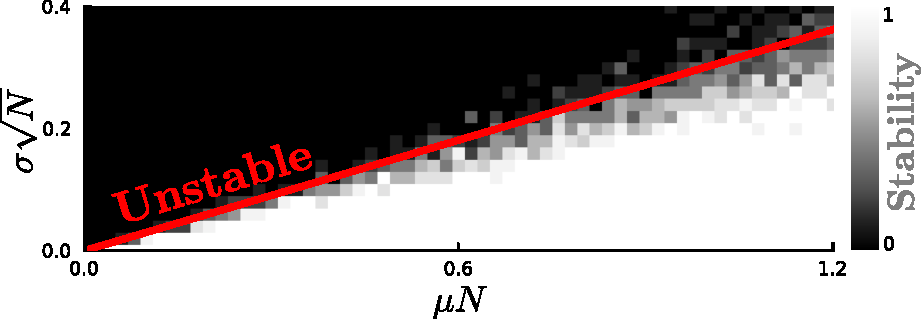
\includegraphics[width=.45\textwidth]{figs/beta1_5-S50-N10-diversity.pdf}
    \caption{For a system in the "anti-May" phase an increase in $N$,
    corresponding to moving along $\sqrt{N}$ in the $(\sigma \sqrt{N},\mu N)$ plane,
    will be stabilizing. Here we show results from simulation of system~\eqref{eq: full abg},
    where stability is defined as full stable coexistence, overleyed with the critical line
    obtained through the cavity method starting from Eq.\eqref{eq: random-stability int} 
    (see main text). The values of the parameters are $\alpha=1$, $\beta=1.5$,
    $\gamma=1$, $N=50$ and $10$ replicates for the simulations.}
    \label{fig: stability line + sims}
\end{figure}

Figure~\ref{fig: alpha-beta} portrays results of simulaitons 
for $\sigma_c\sqrt{N}$ in the $(\alpha,\beta)$ plane, 
at fixed $\mu N$ and $\gamma = 1$ (further details in caption), 
defined as the value above which
full stable coexistence (i.e. 'stability'
as defined for Fig.\ref{fig: stability line + sims}) 
is less probable than $50\%$.
In these simulations we are using $\mu_s = \mu$, which result
in unstable outcomes for $\beta<\alpha$ while
a certain degree of heterogeneity in the interactions
admits admits stability for $\beta>\alpha$, the higher
the larger is the difference between $\beta$ and $\alpha$.
Notice that the existence of a $\sigma_c\sqrt{N}$ above which
instability is triggered does not imply that increasing $N$ will
destabilize the system, because also $\mu N$ would change.
Rather, for all the value of $\beta$ and $\alpha$ in the
upper triangle, the picture is the same as the one depicted in 
Fig.~\ref{fig: stability line + sims}: we are in "anti-May"
phase.

\begin{figure}[h!]
    \centering
    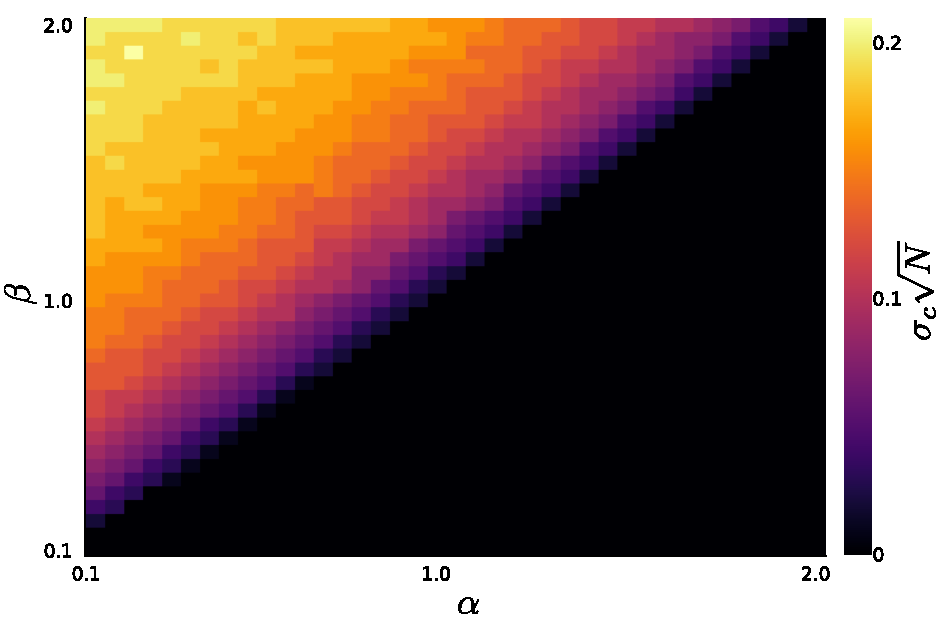
\includegraphics[width=.45\textwidth]{figs/alpha-beta.pdf}
    \caption{The "May" and "anti-May" phases described for the
    case of uniform interactions are robust for random interactions.
    Here we simulated system~\eqref{eq: full abg} for a fixed value of
    $\mu=\mu_s=10^{-2}$, $\gamma=1$, $N=100$ and $100$ replicates 
    and evaluated $\sigma_c$, defined here as
    the value above which full stable coexistence is less probable than 50\%,
    at varying $\alpha$ and $\beta$. No amount of heterogeneity is allowed in the
    lower triangle because we have $\mu=\mu_s$, while an increasing value of $\sigma_c$
    is found as $\beta$ becomes bigger than $\alpha$.
    We stress that the existence of a finite $\sigma_c\sqrt{N}$ above which
    instability is triggered also in the upper triangle,
    does not imply that increasing $N$ will
    destabilize the system, because also $\mu N$ would change (see main text).
    }
    \label{fig: alpha-beta}
\end{figure}
    


\section{Conclusions}

\clearpage

\bibliography{general-stability-bib}

\bibliographystyle{unsrt}

\end{document}
%
% ****** End of file apssamp.tex ******

